% Unofficial University of Cambridge Poster Template
% https://github.com/andiac/gemini-cam
% a fork of https://github.com/anishathalye/gemini
% also refer to https://github.com/k4rtik/uchicago-poster

\documentclass[final]{beamer}

% ====================
% Packages
% ====================

\usepackage[T1]{fontenc}
\usepackage{lmodern}
\usepackage[orientation=portrait,size=a2,scale=1.15]{beamerposter}
\usetheme{gemini}
\usecolortheme{nott}
\usepackage{graphicx}
\usepackage{booktabs}
\usepackage{tikz}
\usepackage{pgfplots}
\pgfplotsset{compat=1.14}
\usepackage{anyfontsize}


% ====================
% Lengths
% ====================

% If you have N columns, choose \sepwidth and \colwidth such that
% (N+1)*\sepwidth + N*\colwidth = \paperwidth
\newlength{\sepwidth}
\newlength{\colwidth}
\setlength{\sepwidth}{0.025\paperwidth}
\setlength{\colwidth}{0.45\paperwidth}

\newcommand{\separatorcolumn}{\begin{column}{\sepwidth}\end{column}}

% ====================
% Title
% ====================

\title{PACE 2024: OCMu64, reductions and a branch-and-bound solver for\\ One-sided Crossing Minimization}

\author{Ragnar {Groot Koerkamp} \inst{1} \and Mees de vries \inst{2}}


\institute[shortinst]{\inst{1} ETH Zurich, @curious\_coding \samelineand
  \inst{2} Unaffiliated, The Netherlands}

% ====================
% Footer (optional)
% ====================

%% \footercontent{
%%   \href{https://utfpr.edu.br/ct/ppgca}{utfpr.edu.br/ct/ppgca} \hfill
%%   Mostra de Trabalhos do PPGCA --- TechTalks 2024 \hfill
%%   \href{mailto:ppgca-ct@utfpr.edu.br}{ppgca-ct@utfpr.edu.br}}
% (can be left out to remove footer)


% ====================
% Logo (optional)
% ====================

% use this to include logos on the left and/or right side of the header:
%% \logoright{\includegraphics[height=2.5cm]{logos/utfpr-logo.png}}
%% \logoleft{\hspace{20ex}\includegraphics[height=3.5cm]{logos/ppgca-logo.png}}

% CUSTOM MACROS

\usepackage{cleveref}
\usepackage{amsthm}
\theoremstyle{remark}
\newtheorem*{remark}{Remark}

\newcommand{\R}{\mathbb R}
\renewcommand{\b}{\prec}
\newcommand{\be}{\preceq}
\newcommand{\g}{\bullet}
\renewcommand{\u}{\overline{u}}
\renewcommand{\v}{\overline{v}}
\DeclareMathOperator{\supp}{supp}

\newcommand{\mees}[1]{{\color{blue}[{\bf{Bryce:}} #1]}}
\newcommand{\ragnar}[1]{{\color{orange}[{\bf{Ragnar:}} #1]}}

% ====================
% Body
% ====================

\begin{document}

% Refer to https://github.com/k4rtik/uchicago-poster
% logo: https://www.cam.ac.uk/brand-resources/about-the-logo/logo-downloads
% \addtobeamertemplate{headline}{}
% {
%     \begin{tikzpicture}[remember picture,overlay]
%       \node [anchor=north west, inner sep=3cm] at ([xshift=-2.5cm,yshift=1.75cm]current page.north west)
%       {\includegraphics[height=7cm]{logos/unott-logo.eps}};
%     \end{tikzpicture}
% }

% Try also: alertblock, exampleblock
% \heading

\begin{frame}[t]
  \begin{columns}[t]
    \separatorcolumn
    \begin{column}{\colwidth}

      \begin{block}{One-sided crossing minimization}
        Given is a bipartite graph $(A, B)$ that is drawn in the plane at points
        $(i, 0)$ and $(j,1)$ for components $A$ and $B$ respectively. The ordering of $A$
        is fixed. The goal is the find an ordering of $B$ that minimizes the number of
        crossings when edges are drawn as straight lines.

        We use $<$ to compare vertices in $A$ in their fixed ordering.
        For $u\in B$, we write $N(u) \subseteq A$ for the set of its neighbours.

        The \textbf{crossing number} $c(u, v)$ is $\sum_{(a, b) \in A^2}
        u(a)v(b)[a > b]$, the number of
        crossings between edges incident to $u$ and $v$ when $u$ is drawn before $v$.  For
        $X,Y\subseteq B$ we set $c(X,Y) = \sum_{x\in X}\sum_{y\in Y} c(x,y)$ for the cost of ordering
        all vertices of $X$ before all vertices of $Y$. More generally, $c(X,Y,Z) = c(X, Y) + c(X, Z) +
        c(Y, Z)$. We also consider the \emph{reduced cost} $r(X,Y) = c(X, Y) - c(Y, X)$, which is
        negative when $X$ is better \emph{before} $Y$ and positive when $X$ is better \emph{after} $Y$.

        We write $u\b v$ when $u$ must come before $v$ in \emph{all} minimal solutions, and say that $(u, v)$
        is a \textbf{fixed pair}.
        We try to fix as many pairs as possible to speed up the search.
        A well known result is that when $\max N(u) < \min N(v)$, then $u\b v$.

        \vspace{-1.5em}
        \centering
        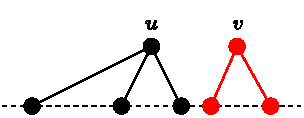
\includegraphics[scale=2]{fig/simple.pdf}
      \end{block}

      \begin{block}{Strongly fixed pairs}
        We call $u, v \in B$ a \textbf{strongly fixed pair} if $N(u) \neq N(v)$
        and their degrees are $n$
        and $m$ and for all $0 \leq i < n$,
        $$N(u)_i \leq N(v)_{\lfloor i\cdot m/n \rfloor}.$$
        That is: for all $x$, \emph{the $x\%$'th neighbour of $u$ is left of the $x\%$'th
        neighbour of $v$}.
        %% Note that this implies $r(u, v) < 0$.

        \begin{center}
          \vspace{-2em}
        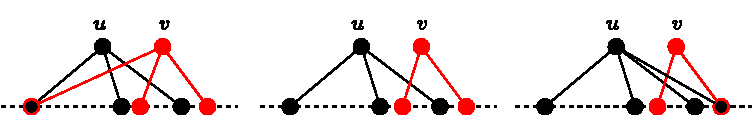
\includegraphics[scale=1.5]{fig/strongly-fixed.pdf}
          \vspace{-2em}
        \end{center}

        \textbf{Main result:}
        If $(u, v)$ is strongly fixed, then $u \b v$.

        \textbf{The lemma is optimal:}
        Without further assumptions on $(A, <)$ or on the other elements of $B$, it is not
          possible to prove $u \b v$ if $(u, v)$ is not strongly fixed.
        Suppose that $u, v \in B$ with $N(u) \neq N(v)$ are not strongly fixed, and let $i$ be
        such that $b:=N(u)_i > N(v)_{\lfloor i\cdot m/n\rfloor}=:a$. Now take sets of vertices $L, M,
          R \subseteq A$ with $a < M < b$, with $L < \min(N(v))$ and with
          $\max(N(u)) < R$.
          Add a node $x \in B$ connected to $L$, $M$, $R$. With the correct numbers of vertices in
          $L$, $M$, $R$ we can make it so that $c(v, x, u) < \min(c(x, u, v), c(u, v, x))$, so that
        $v$ has to go before $u$.

        \centering
          \vspace{-0.5em}
        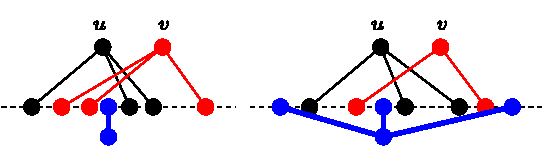
\includegraphics[scale=1.5]{fig/blocking-set.pdf}
          \vspace{-1em}
      \end{block}

      \begin{block}{Practically fixed pairs}
        Although such a node $x$ may exist in theory, it does
        not have to exist in the actual set $B$, motivating a more practical approach:

        \textbf{Blocking set:}
        Suppose $r(u,v)< 0$, i.e., $u$ wants to go left of $v$.
        A \emph{blocking set} $X\subseteq B-\{u,v\}$ is a set such that $c(v,X,u) \leq \min(c(v, u,
        X), (X, v, u))$.  If there is no blocking set for $(u, v)$, we call it a
        \emph{practically fixed pair}, and $u\b v$.
      \end{block}

      \textbf{Finding blocking sets:}
      Such a set $X$ can be found, if one exists, using a knapsack-like algorithm: for
      each $x\in B-\{u,v\}$, add a point $P_x = (r(v, x), r(x, u))$, and search for a subset summing
      to ${\leq{}(r(u, v), r(u, v))}$.

      %% Note that we do not require $(v, X, u)$ to be a true local minimum, since we do
      %% not consider interactions between vertices in $X$, as that would make ruling out the
      %% existence of such sets much harder.

      %% \begin{block}{Weak variants}
      %%   It is also possible to consider \emph{weak} variants of the above lemmas that
      %%   only imply that $u < v$ in \emph{some} optimal solution. This requires careful
      %%   handling of cycles like $u\be v\be w\be u$.
      %% \end{block}
    \end{column}

    \separatorcolumn

    \begin{column}{\colwidth}
      \begin{block}{Gluing}
        When $u$ and $v$ are consecutive in \emph{all} optimal solutions,
        we \textbf{glue} them together and treat them as a single vertex.

        \textbf{Identical nodes:}
        When $u$ and $v$ have the same neighbours, we glue them.

        \begin{center}
          \vspace{-1em}
        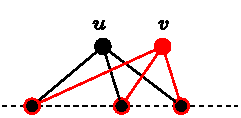
\includegraphics[scale=2]{fig/gluing.pdf}
        \end{center}

        \textbf{Greedy gluing:}
        When $r(u, x)\leq 0$ for all $x\in B$, there is a solution that
        starts with $u$.

        \textbf{Practical gluing lemma (unused):}
        Let $u$ and $v$ satisfy $r(u, v) \leq 0$.
        A non-empty subset $X\subseteq B-\{u,v\}$ is \emph{blocking} when $c(u, X, v) \leq
        \min(c(u, v, X), c(X, u, v))$. If there is no blocking set, then we can glue $u, v$.

        Again such sets $X$ can be found or proven to not exist using a knapsack
        algorithm: add points $P_x = (r(u, x), r(x, v))$ and search for a non-empty
        set summing to $\leq{}(0,0)$.
      \end{block}

      \begin{block}{Solver}
        Our solver \texttt{OCMu64} uses a standard \textbf{branch-and-bound on the ordering of the
        solution}.  We start with fixed prefix $P=()$ and tail $T=B$, and in each step we try (a
        subset of) all vertices in $T$ as the next vertex appended to $P$.
        In a preprocessing step we compute the trivial lower bound $S_0 =
        \sum_{u,v}\min(c(u,v),c(v,u))$ on the score.
        %% We keep track of the score $S_P$ of the prefix and $S_{PT}=c(P, T)$ of
        %% prefix-tail intersections, and abort when this score goes above the best
        %% solution found so far.

        \begin{description}
        \item[Graph simplification]
          %% We drop degree-$0$ vertices, merge identical
          %% vertices, and split the graph into \emph{independent} components.
          The initial solution uses the median heuristic followed by a simple local search that tries to move
          slices and optimally insert them.
          We then re-label all nodes in order to make memory accesses more efficient.
        \item[Fixed pairs] We find all strongly fixed pairs and store them. For the
          exact track we also find practically fixed pairs.
          For each tail we search for \emph{tail-local} practically fixed pairs. In each state, we only
          try vertices $u\in T$ not fixed after another $v\in T$.
        \item[Gluing\quad] We use the greedy gluing strategy. Our implementation
          of practical gluing contained a bug, so we did not use this.
        \item[Tail cache] In each step, we search for the longest suffix of $T$ that
          was seen before, and reuse (the lower bound on) its score. We also
          cache the tail-local practically fixed pairs.
        \item[Optimal insert] Instead of simply appending $u$ to $P$, we
          insert it in the optimal position. The
          implementation is tricky because it interacts in complicated ways with
          the caching of results for each tail.
        \end{description}
      \end{block}

      \begin{block}{Performance}
        \textbf{Parameterized track:} All 200 instances in \textbf{10.37s} total
        time (second place).

        \textbf{Exact track:} 157/200 instanes.

      \end{block}

      %% \begin{block}{References (optional)}
      %%   \nocite{*}
      %%   \footnotesize{\bibliographystyle{plain}\bibliography{poster}}
      %% \end{block}

    \end{column}
    \separatorcolumn
  \end{columns}
\end{frame}

\end{document}
